%% ----------------------------------------------------------------------------
% BIWI SA/MA thesis template
%
% Created 09/29/2006 by Andreas Ess
% Extended 13/02/2009 by Jan Lesniak - jlesniak@vision.ee.ethz.ch
%% ----------------------------------------------------------------------------
\newpage
\chapter{Discussion}
\label{ch:discussion}
In the previous section it has become evident that CNNs are very well capable of learning the ordering task, both the simple 3-input binary task reaching up to 82.8\% accuracy as well as the 4-input 24-output permutation version with an top-1 accuracy of 59.3\% using interpolated lidar depth. Especially the accuracy on the OPN4 network is remarkably high, given the fact that even a single swap in the estimated order would cause a wrong prediction. From the acquired results it can therefore definitely be concluded that neural networks are very well able to sort video frames acquired from driving cameras, an interesting result for itself. The studied network based on the earlier proposed OPN network \cite{lee2017} apparently scales well to the KITTI dataset and to various feature maps like lidar.

It has been shown that particularly the channel-splitted grayscale image images, the interpolated lidar depth and the estimated lidar height above ground provide strong features for the network to train on. Especially the interpolated lidar depth shows considerable improvement and it is clear that this preprocessing step benefits the learning significantly. Also the color images are strong, as expected, in comparison to the reflectances which apparently do not contain enough information to lead to convergence.

%This mostly follows expectations, although it is interesting to note that color images and the interpolated lidar are features with similar strengths, while the height above ground is superior to both of those.

While the neural networks have definitely shown to be capable learning this task, it interesting to find out what representation the networks actually primarily learn. As the task does not require the detection of any object it is not directly expected that the network only learns to detect a particular class of objects. Can we gain an overview what the backbone network exactly learns? 

\begin{figure}[t]
\centering
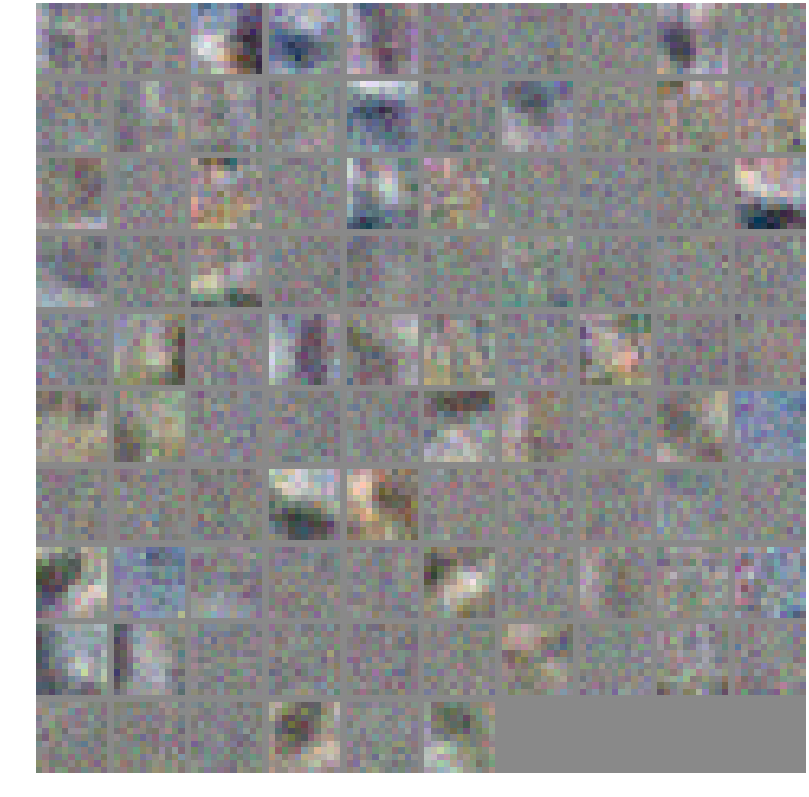
\includegraphics[width=0.49\textwidth]{images/grp0_conv1_weights_color.png}
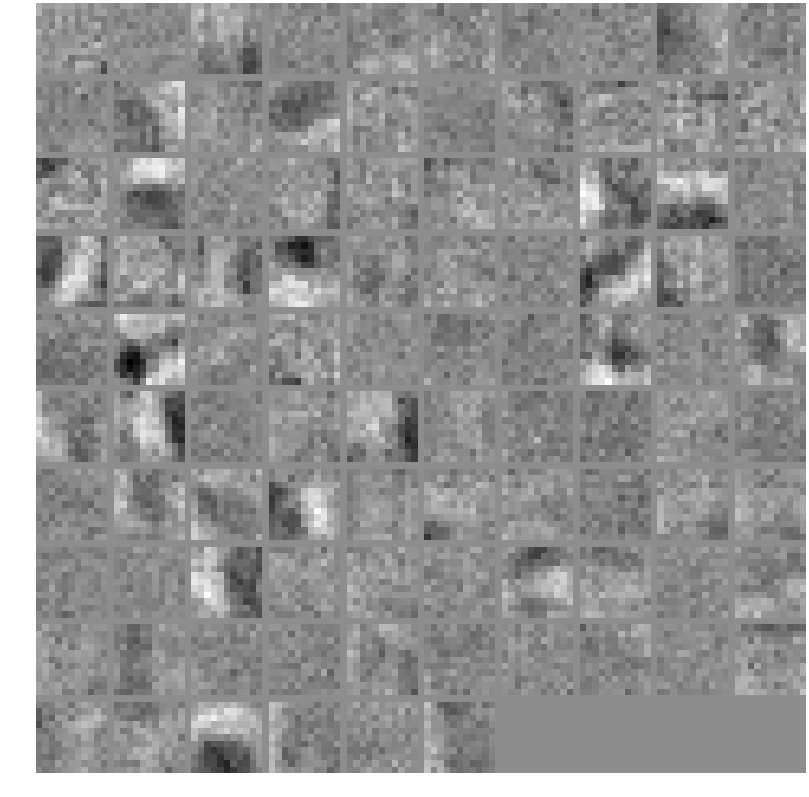
\includegraphics[width=0.49\textwidth]{images/grp0_conv1_weights_gray.png}
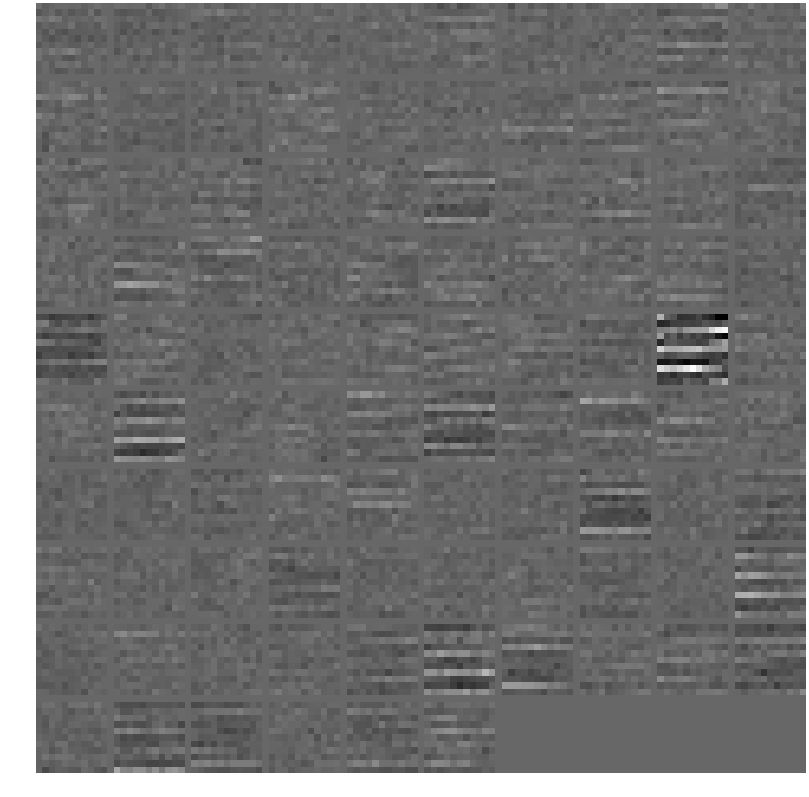
\includegraphics[width=0.49\textwidth]{images/grp0_conv1_weights_lid.png}
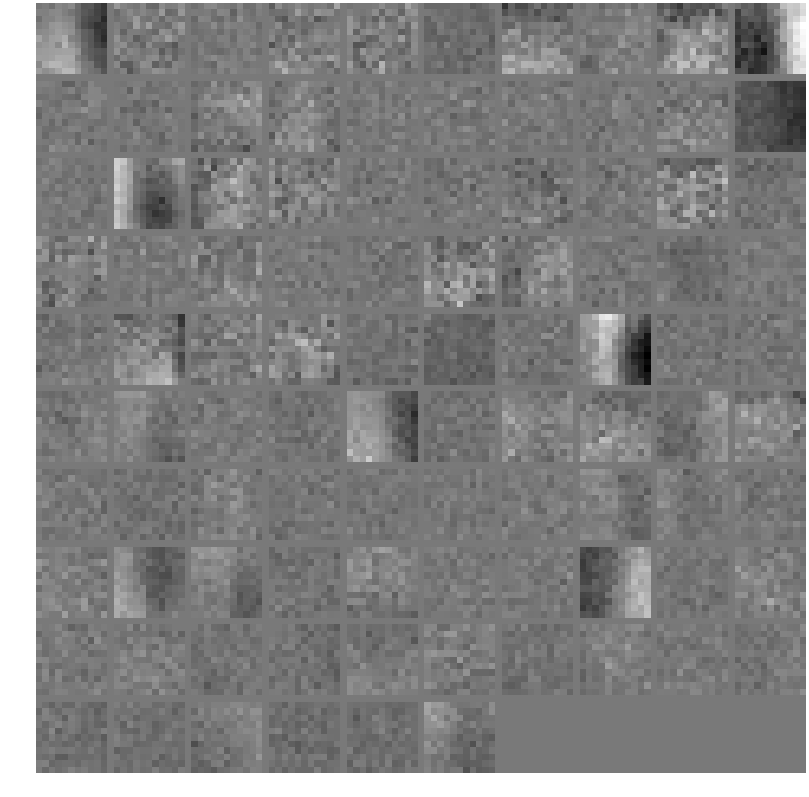
\includegraphics[width=0.49\textwidth]{images/grp0_conv1_weights_lid_depth.png}
\caption{Weights of the first convolutional layer of different feature maps, from top-left to bottom-right: color, grayscale, lidar and interpolated lidar}
\label{fig:filters}
\end{figure}

With the several millions of parameters contained in a neural network, this is not a particularly easy task. However several methods have been developed to visualize neural networks,  The simplest and remarkably effective way to investigate the strength of the learning is to look at the first-order convolutional layers. The filters in those layers are applied directly on the image and they therefore contain first-level patterns the network learns. The first-order filters that are learned from some of the main individual feature maps are shown in Figure \ref{fig:filters}. Note first that all of the maps, except the images from the color camera, do only have one layer and are therefore shown in grayscale. The activations resulting from the grayscale images are provided in Appendix \ref{app:additional_visualizations} for reference.

It is immediately clear that several general filters are learned, but the filters are not all strong and some are relatively noisy. Focusing on the filters from the color images, it is clear that those color images do not really add significant information compared to the grayscale versions, as there are barely real color filters and instead mostly structural filters in several color variations. Only one blue filter is present, which appears to trigger on the sky. On the lidar filters the strength of the interpolation preprocessing is apparent, the non-interpolated version has only some noisy ribbed filters, showing the apparent complexity of handling the preprocessing with the network. In any case, for all networks more than half of the filters are considered 'dead' as they only contain a noise pattern. Thus only some edge and corner filters are learned, suggesting that a limited number of filters is apparently adequate for solving the task. This is especially visible with the interpolated filters, that contain mostly low-level filters with only vertical edges, indicating that these are apparently sufficient. Thus while the networks perform well on this data source, the task may actually be too easy to learn a rich representation from this feature map.
%Approximately half of the filters can however be considered 'dead' as they contain only a noise pattern, from which it appears only a limited number of filters is apparently adequate for solving the task.

\begin{figure}[t]
\centering
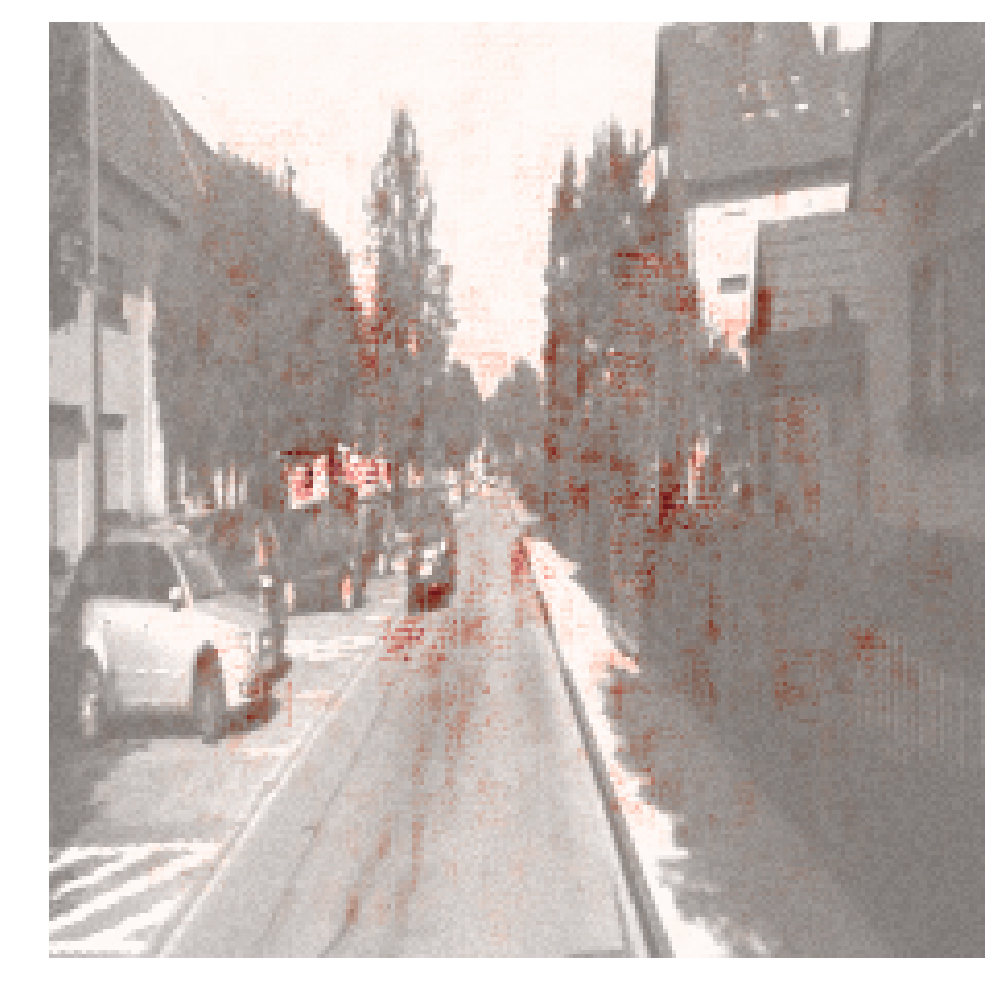
\includegraphics[width=0.49\textwidth]{images/saliency_1-0.png}
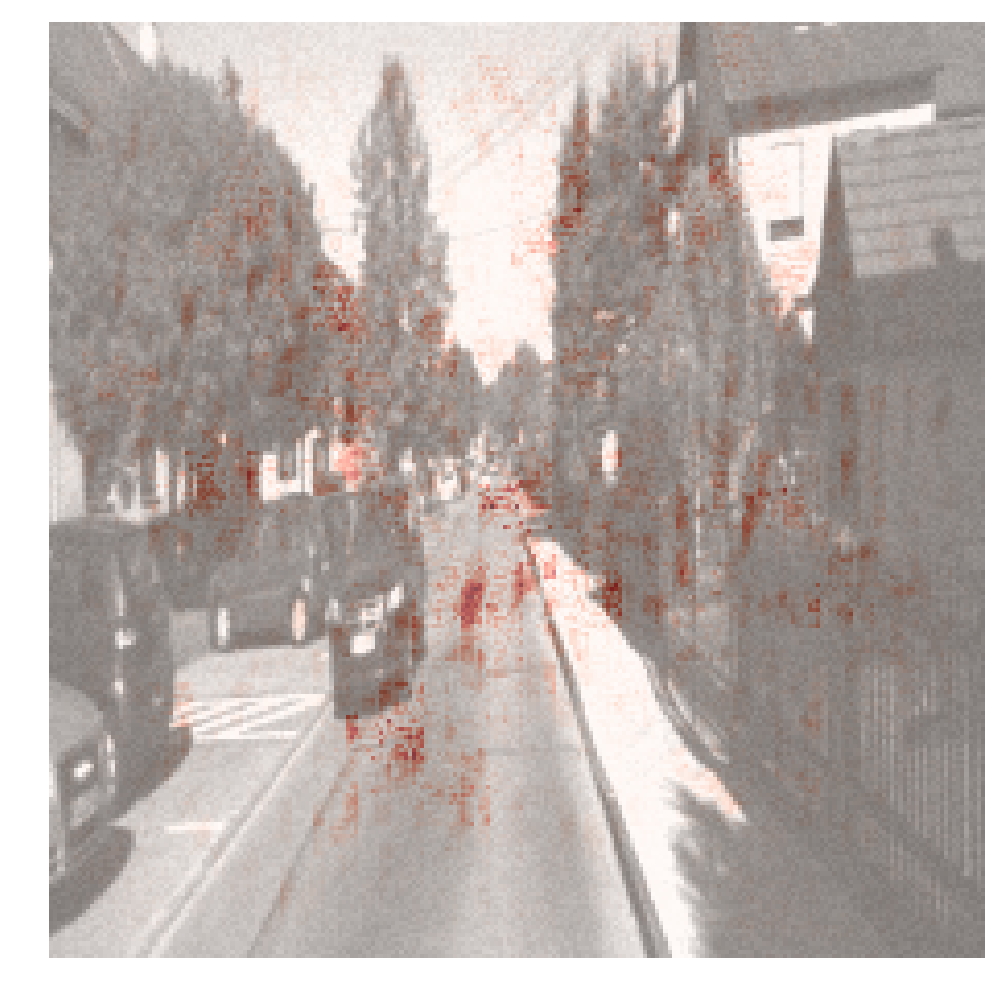
\includegraphics[width=0.49\textwidth]{images/saliency_1-1.png}
\caption{Saliency maps on the grayscale feature maps of two frames in the sequence shown in Figure \ref{fig:frames}, the darker the red color the stronger the pixel influences the output permutation}
\label{fig:saliency}
\end{figure}

To investigate in more detail where the network focuses on, an alternative visualizing technique is investigated: saliency maps. Figure \ref{fig:saliency} shows saliency maps on the grayscale version in two frames. The saliency map should give an indication of the most important part of the image, but it is evident that the saliency map does not show particular attention to a certain kind of high-level feature, for example cars. There is also not a very apparent overlap between the same objects tracked through multiple frames in the sequence. The most important part of the image often appear at the center of every single frame, but this could have been anticipated as those parts should appear in multiple frames making it possible to compare them. It could however also suggest that a zoom-in might be used directly to compare the frames. This could indicate that the sequences have too little dynamic movement, as it appears that the network is partly ignoring the moving car, and instead finds the parts which remain static in both images. It should however be noted that the saliency maps do not appear to have been applied in this context before and there exists therefore no relevant literature to verify the applicability of this approach for this task. An alternative approach which also shows similar highlights in the area is given in Appendix \ref{app:additional_visualizations}.

Directly correlating corresponding parts in the image would be an foreseen approach, but it is is not expected to be so efficient, given the complex movement around the streets, with cars passing in the other direction, traffic crossing the street and the car turning in turns. While the saliency map seems to indicate that the indirect correlation approach comparing the relatively simple patterns learned from the backbone network between the different images might be a strong approach, this does not explain the high accuracy in turns reported in the previous section, because direct correlation of a zoom-in version does not work in that respect. 

%but this picture seems to indicate that the indirect correlation approach comparing the relatively simple patterns learned from the backbone network between the different images might still be a strong approach. It is however hard to conclude this confidently, as the saliency maps do not necessarily give the complete picture. Moreover, this technique has not been applied in this context before and there exists therefore no relevant literature to verify the applicability of this approach in this context.

\begin{figure}[t!]
\centering
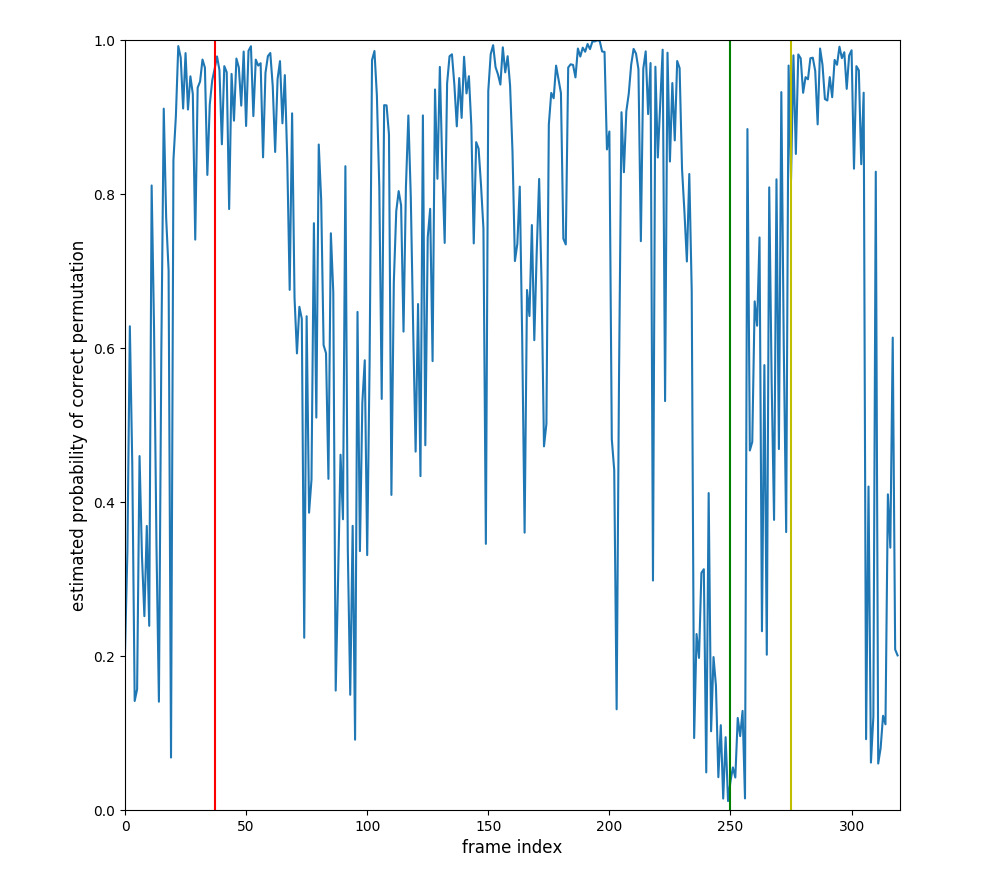
\includegraphics[width=\textwidth]{images/percentages_small.png}
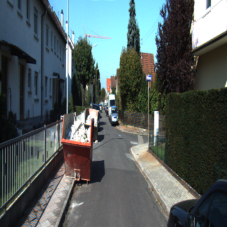
\includegraphics[width=0.32\textwidth]{images/000037.png}
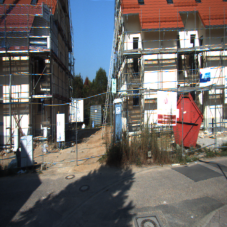
\includegraphics[width=0.32\textwidth]{images/000250.png}
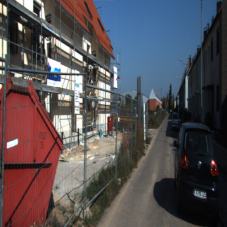
\includegraphics[width=0.32\textwidth]{images/000275.png}
\caption{Estimated probability of the sorted order of 4 frames of interpolated lidar depth given as input from the first 320 frames of sequence 15 with the index indicating the number of the first frame (top). On the bottom three images are shown with the left corresponding to the red line, the second to the green line and the third one to the yellow line}
\label{fig:percentages}
\end{figure}

To check the performance in different conditions a new test set has been created, starting at every frame from a particular sequence in sorted order. The probability is measured that the network correctly confirms that the frames are sorted (note that giving the items in sorted order might appear like an easier task, but the network has not been trained with any preference for sorted sequences). The result on the first 320 frames of sequence 15 are shown in Figure \ref{fig:percentages}. From the graph it clearly follows that there are  sections in the sequence where the network performs better (reaching close to 100\% accuracy) and worse, but there are also sections where the probability has sudden peaks. Color images of three frames in the sequence are also shown (please note that the data itself is trained on the interpolated lidar depth). It is not directly trivial to see why the specified sections are easy or hard. In the first image showing a region with high accuracy the network seems to work well around the red storage box, but it would be highly unlikely the network focuses on storage boxes. At the end of the road the accuracy is low, possibly due to the lack of a proper road (with a house under construction instead). Between the second and third image the car is turning, from which it is clear that during the turn results are bumpy, but still better than before the turn. Afterwards strong results are achieved for a certain time span, but it is again not obvious what makes this part easier. 

Several techniques to visualize the behavior of the neural network were attempted, but it remains difficult to get a deeper understanding of the performance of the network. Therefore it is unfortunately hard to conclude where the relatively strong performance on the task exactly comes from. The learned filters show some generic patterns, but seem in general of limited strength and that makes it questionable if the network in the current state could be adopted for fine-tuning.


%A similar approach to find the important regions on the image is to find the location of the maximal activated neurons in the higher layers, for example in the fifth convolutional layer. For comparison with the previous approach the 5 maximal regions are shown for one of the frames investigated with the saliency map is shown in Figure \needfig. It is again hard to point which features the network is exactly focusing on, but there seems again a general tendency on several general static objects, for example trees around and the contour in the road. It remains however difficult to generalize a particular feature over multiple frames.
